%%%%%%%%%%%%%%%%%%%%%%%%%%%%%%%%%%%%%%%%%%%%%%%%%%%%%%%%%%%%%%%%%%%%%%%%%%%
%% This file is part of the book
%%
%% Algorithmic Graph Theory
%% http://code.google.com/p/graph-theory-algorithms-book/
%%
%% Copyright (C) 2009--2011 Minh Van Nguyen <nguyenminh2@gmail.com>
%%
%% See the file COPYING for copying conditions.
%%%%%%%%%%%%%%%%%%%%%%%%%%%%%%%%%%%%%%%%%%%%%%%%%%%%%%%%%%%%%%%%%%%%%%%%%%%

\documentclass{article}

\usepackage{subfigure}
\usepackage{tikz}
\usetikzlibrary{external}
\tikzexternalize{maze-graph}

\begin{document}

\begin{figure}
%% a maze
\subfigure[]{
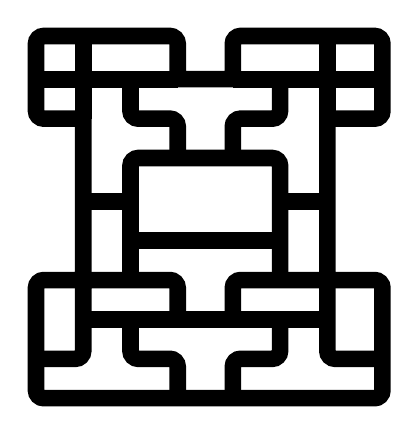
\begin{tikzpicture}
[cornerJagged/.style={rounded corners=0cm},%
  cornerRounded/.style={rounded corners=0.1cm},%
  invisibleNode/.style={},%
  pathDecorate/.style={-,line width=6pt}]
%% invisible nodes or vertices
%% \foreach \nodename/\x/\y in {1/0.1/0.6, 2/4.5/0.6, 3/1.9/0.1,
%%   4/2.6/0.1, 5/0.7/1.1, 6/1.3/1.1, 7/1.9/1.1, 8/2.6/1.1, 9/3.2/1.1,
%%   10/3.8/1.1, 11/0.7/1.6, 12/1.3/1.6, 13/3.2/1.6, 14/3.8/1.6,
%%   15/1.3/2.1, 16/3.2/2.1, 17/0.7/2.6, 18/1.3/2.6, 19/3.2/2.6,
%%   20/3.8/2.6, 21/1.9/3.15, 22/2.6/3.15, 23/0.7/3.65, 24/3.8/3.65,
%%   25/0.1/4.15, 26/0.7/4.15, 27/1.3/4.15, 28/1.9/4.15, 29/2.6/4.15,
%%   30/3.2/4.15, 31/3.8/4.15, 32/4.5/4.15, 33/0.7/4.7, 34/3.8/4.7,
%%   35/0.1/0.1, 36/4.5/0.1, 37/0.7/0.6, 38/1.3/0.6, 39/1.9/0.6,
%%   40/2.6/0.6, 41/3.2/0.6, 42/3.8/0.6, 43/0.1/1.6, 44/1.9/1.6,
%%   45/2.6/1.6, 46/4.5/1.6, 47/1.3/3.15, 48/3.2/3.15, 49/0.1/3.65,
%%   50/1.3/3.65, 51/1.9/3.65, 52/2.6/3.65, 53/3.2/3.65, 54/4.5/3.65,
%%   55/0.1/4.7, 56/1.9/4.7, 57/2.6/4.7, 58/4.5/4.7}
%% {
%%   \node (\nodename) at (\x,\y) [invisibleNode] {};
%% }
%% edges or lines representing the path of the maze
%% the outer path
\draw[pathDecorate] (0.1,0.1)[cornerRounded] -- (4.5,0.1) --
(4.5,1.6)[cornerJagged] -- (3.8,1.6) -- (3.8,3.65)[cornerRounded] --
(4.5,3.65) -- (4.5,4.7) -- (2.6,4.7)[cornerJagged] -- (2.6,4.152) --
(1.9,4.152)[cornerRounded] -- (1.9,4.7) -- (0.1,4.7) --
(0.1,3.65)[cornerJagged] -- (0.7,3.65) -- (0.7,1.6)[cornerRounded] --
(0.1,1.6) -- cycle;
%% inner paths
\draw[pathDecorate] (0.1,0.6)[cornerRounded] --
(0.7,0.6)[cornerJagged] -- (0.7,1.6)[cornerRounded] -- (1.9,1.6) --
(1.9,1.1);
\draw[pathDecorate] (0.7,1.1) -- (3.8,1.1);
\draw[pathDecorate] (1.3,1.1)[cornerRounded] -- (1.3,0.6) -- (1.9,0.6)
-- (1.9,0.1);
\draw[pathDecorate] (2.6,0.1)[cornerRounded] -- (2.6,0.6) -- (3.2,0.6)
-- (3.2,1.1);
\draw[pathDecorate] (2.6,1.1)[cornerRounded] -- (2.6,1.6) -- (3.8,1.6);
\draw[pathDecorate] (3.8,1.6)[cornerRounded] -- (3.8,0.6) -- (4.5,0.6);
\draw[pathDecorate] (1.3,1.6)[cornerRounded] -- (1.3,3.15) --
(3.2,3.15) -- (3.2,1.6);
\draw[pathDecorate] (1.3,2.1) -- (3.2,2.1);
\draw[pathDecorate] (0.7,2.6) -- (1.3,2.6);
\draw[pathDecorate] (3.2,2.6) -- (3.8,2.6);
\draw[pathDecorate] (0.1,4.15) -- (1.9,4.15);
\draw[pathDecorate] (2.6,4.15) -- (4.5,4.15);
\draw[pathDecorate] (0.7,3.65) -- (0.7,4.7);
\draw[pathDecorate] (3.8,3.65) -- (3.8,4.7);
\draw[pathDecorate] (1.3,4.15)[cornerRounded] -- (1.3,3.65) --
(1.9,3.65) -- (1.9,3.15);
\draw[pathDecorate] (2.6,3.15)[cornerRounded] -- (2.6,3.65) --
(3.2,3.65) -- (3.2,4.15);
\end{tikzpicture}
}
\qquad
%%
%% graph representation of maze
\subfigure[]{
\label{fig:maze_graph:graph_representation}
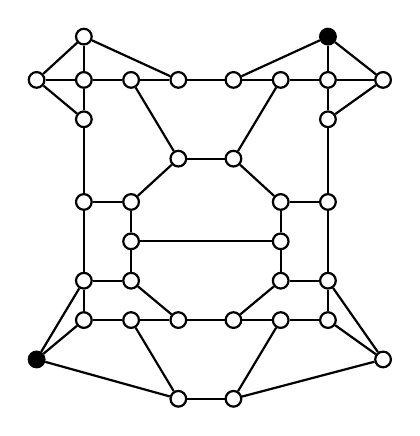
\begin{tikzpicture}
[linedecorate/.style={-,thick},%
  nodeBlackFilled/.style={shape=circle,fill=black,inner sep=2pt,draw,thick},%
  nodeHollow/.style={shape=circle,inner sep=2pt,draw,thick}]
%% nodes or vertices
\foreach \nodename/\x/\y in {2/4.5/0.6, 3/1.9/0.1,
  4/2.6/0.1, 5/0.7/1.1, 6/1.3/1.1, 7/1.9/1.1, 8/2.6/1.1, 9/3.2/1.1,
  10/3.8/1.1, 11/0.7/1.6, 12/1.3/1.6, 13/3.2/1.6, 14/3.8/1.6,
  15/1.3/2.1, 16/3.2/2.1, 17/0.7/2.6, 18/1.3/2.6, 19/3.2/2.6,
  20/3.8/2.6, 21/1.9/3.15, 22/2.6/3.15, 23/0.7/3.65, 24/3.8/3.65,
  25/0.1/4.15, 26/0.7/4.15, 27/1.3/4.15, 28/1.9/4.15, 29/2.6/4.15,
  30/3.2/4.15, 31/3.8/4.15, 32/4.5/4.15, 33/0.7/4.7}
{
  \node (\nodename) at (\x,\y) [nodeHollow] {};
}
\node (1) at (0.1,0.6) [nodeBlackFilled] {};
\node (34) at (3.8,4.7) [nodeBlackFilled] {};
%% edges or lines
\path
\foreach \startnode/\endnode in {1/3, 1/5, 1/11, 2/4, 2/10, 2/14, 3/4,
  3/6, 4/9, 5/6, 5/11, 6/7, 7/8, 7/12, 8/9, 8/13, 9/10, 10/14, 11/12,
  11/17, 12/15, 13/14, 13/16, 14/20, 15/16, 15/18, 16/19, 17/18,
  17/23, 18/21, 19/20, 19/22, 20/24, 21/22, 21/27, 22/30, 23/25,
  23/26, 24/31, 24/32, 25/26, 25/33, 26/27, 26/33, 27/28, 28/29,
  28/33, 29/30, 29/34, 30/31, 31/32, 31/34, 32/34}
{
  (\startnode) edge[linedecorate] node {} (\endnode)
};
\end{tikzpicture}
}
\end{figure}

\end{document}
